\section{Evaluation}
The following subsections evaluate the project in visual realism.
They further discuss the possibilities to measure realism or approximate such a value.

\subsection{Visual Realism}
\label{section:techimpl:measure}
Since this project renders cloudscapes based on real weather forecasts, the clouds are supposed to look as realistic as possible.
To assess the realism of the rendered image, several aspects have to be considered.
\\
First is the tone mapping of the image. The human eye is adapted to natural colors and quickly detects disparities in a color palette that does not reflect Nature's colors.
\\
According to Rademacher \cite{diglib:realism}, the shadow softness of cast shadows is a also great way of determining how realistic a rendered image looks.
Apparently, the same is true for surface smoothness.
Unfortunately, both these techniques are not applicable as the clouds have no smooth surface and the shadow is cast on a vibrantly colored terrain, making it hard to read where shadows start and end.
\\
Rademacher makes another good point, which relates to the simplicity of the scene.
He states that "[...] in a rendering application, it may be better to spend time on generating proper soft shadows and adequate textures, rather than adding more of the same lights
or objects, or simply adding new objects for variety" \cite{diglib:realism2}.
\\
This leaves to believe that in order to achieve higher fidelity and realism, the focus should be put on the texturing and shadow casting of the clouds, rather than the shape and quantity.
\emptyline
Still, there are some other methods involving \gls{neuralnetwork}s that try to interpret the realism of a rendered image.

\subsubsection{Convolutional Neural Network}
Given there is a \gls{cnn} that is able to classify images of the sky, the weather or clouds into descriptive labels or even genera of cloud formations, then one could just seed those rendered images into the CNN and verify whether the results are truthfully showing "real" clouds.
Of course, this is heavily dependent of how well the \gls{cnn} was trained.

\subsubsection{Generative Adversarial Network}
A similar approach to the \gls{cnn} is a \gls{gan} setup. It describes two neural networks, which compete with each other in a cat-and-mouse game: The \textit{generative} network tries to imitate the training set by generating artificial photographs with many realistic characteristics, while the \emph{discriminative} network tries to tell whether the generated images are fake or not.
\\
With this method, the rendered cloud images could be passed through the discriminative neural network to see if at least the network thinks the images are of real clouds.

\subsubsection{Histogram Comparison}
The \textit{\gls{histogram}} is a graphical representation of data like brightness or color distribution of a given photograph.
When extracting the color \gls{histogram}s of the real photograph and the one of the rendered image, they could be compared and rated how different in color they are.

\subsubsection{Professional Meteorological Assessment}
Another viable solution is to let a professional meteorologist inspect and rate the rendered images and judge the realism of the depicted scenarios, which should reveal if the rendered clouds could actually form and exist in reality.

\subsubsection{Measurability of Realism}
\label{section:eval:measurability}
The previous subsections suggest that there are ways to validate and interpret the visual realism of the rendered images, but no practical method to factually measure that value.
As for this project, the realism of the render output will therefore not be measured, nor quantified or estimated.

\subsection{Physical Accuracy}
It is important to note that the project is only a visualization of weather forecasts, not a physically accurate simulator.
Specifically the formation and dissipation of clouds, the sun's position in the sky, and the wind speed do not necessarily match their real counterparts.

\subsection{Roundshot Image Overlay}
The following graphic shows how the \emph{Roundshot} images are integrated into the weather rendering system.
When the application is running in "real-time mode", which is the mode that visualized the \emph{meteoblue} data, then a button at the bottom of the \gls{ui} lets the user toggle an overlay.
The overlay shows a photograph of the same location and of the corresponding time and date, taken by a \emph{Roundshot} camera.

\begin{figure}[H]
    \centering
    \begin{tikzpicture}[scale=0.8]
        \tikzset{edge/.style = {-{Latex[length=3mm]},shorten >= -4pt}}
        \tikzset{shortedge/.style = {shorten <=-4pt,shorten >= -4pt}}
        \tikzset{icon/.style = {font=\Large}}
        \tikzset{mini/.style = {font=\footnotesize}}
        \tikzset{tiny/.style = {font=\tiny}}

        % cloud layer boxes
        \node[inner sep=0pt] at (7,0.1) 
            {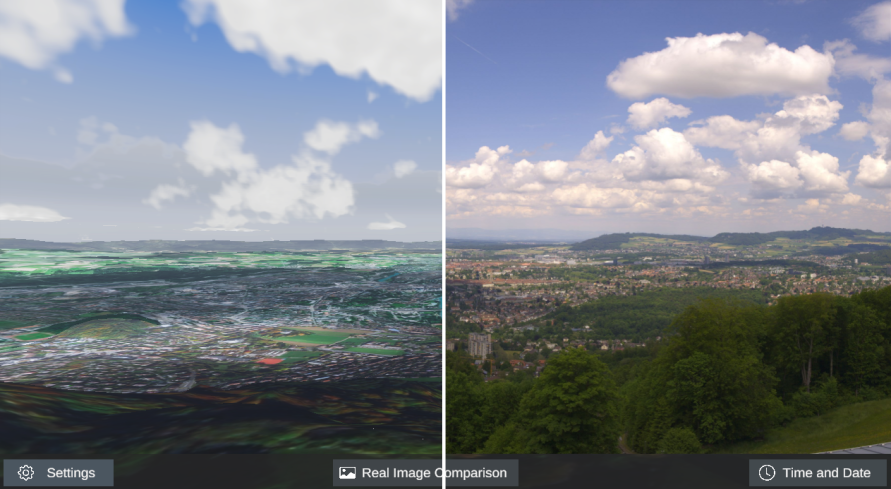
\includegraphics[width=0.8\textwidth]{results/roundshot.png}};

        % tile label 1
        \draw (-0.7,4.6) -- (6.9,4.6);
        \draw (-0.7,4.55) -- (-0.7,4.65);
        \draw (6.9,4.55) -- (6.9,4.65);
        \node at (3.1,4.9) {no overlay};
        
        % tile label 2
        \draw (7,-4.4) -- (14.7,-4.4);
        \draw (7,-4.35) -- (7,-4.45);
        \draw (14.7,-4.35) -- (14.7,-4.45);
        \node at (10.85,-4.7) {overlay active};
        
    \end{tikzpicture}
    \captionof{figure}{Visual comparison of the rendered scene with and without the \emph{Roundshot} image overlay activated.}
    \label{img:results:roundshot}
\end{figure}

\clearpage

\noindent
\autoref{img:results:roundshot} only shows a visual comparison of the two cases where the overlay is activated and where it is not.
In the application, the overlay spans over the whole viewport instead of just half.

\noindent
The comparison brings out a couple of things that are missing in the weather rendering system, but especially that there is room for improvement regarding the cloud shapes.
Also, the cloud colors lack diversity and are too uniform to be naturally realistic.

\subsection{Comparison to Previous Work}
\label{section:techimpl:comparison}
The prototype created in the previous work was able to render a single layer of clouds. There was no \gls{ui} and the scene only contained mockup plants and rocks.
That implementation was able to run at approximately 30 \gls{fps} in Full HD. The \gls{raymarching} and step count was 25, while there were only two steps for the \gls{lightmarching}.
Therefore, the number of texture lookups $s_{previous}$ adds up to a total of:
$$
\begin{array}{l}
    s = n_{layers} * (steps_{ray} * steps_{light}) \\
    s_{previous} = 1 * (25 * 2) = 50
\end{array}
$$

\noindent
The new solution that was achieved in this project has three cloud layers instead of just one.
It also uses 100 steps for \gls{raymarching} and 25 for \gls{lightmarching}.

$$
\begin{array}{l}
    s_{current} = 3 * (100 * 25) = 7500
\end{array}
$$

\noindent
Knowing that the current solution runs at 60 \gls{fps}, this gives an approximate performance gain of factor $(7500 / 50) * (60/30) = 300$.
That is an astounding \textbf{300} times more powerful.
\\
For almost all of this, credit has to be given to the use of a \gls{computeshader}.
The fact that the \gls{noise} has to be calculated only once instead of every frame allows for much higher fidelity in rendering the clouds.

\clearpage

\subsection{Comparison to Other Work}
As it happens, Microsoft's Flight Simulator game (2020) also uses weather data from \emph{meteoblue} to render its \gls{volumetric} clouds \cite{meteoblue:msfs}.
The results are extraordinary and present realistic clouds and weather.

\begin{figure}[H]
    \centering
        \begin{minipage}{0.47\linewidth}
            \includegraphics[width=\linewidth]{results/msfs/2.png}
            \captionof{figure}{Screenshot of Microsoft's Flight Simulator, flying over Bern.}
            \label{img:msfs:1}
        \end{minipage}
    \hfill
        \begin{minipage}{0.47\linewidth}
            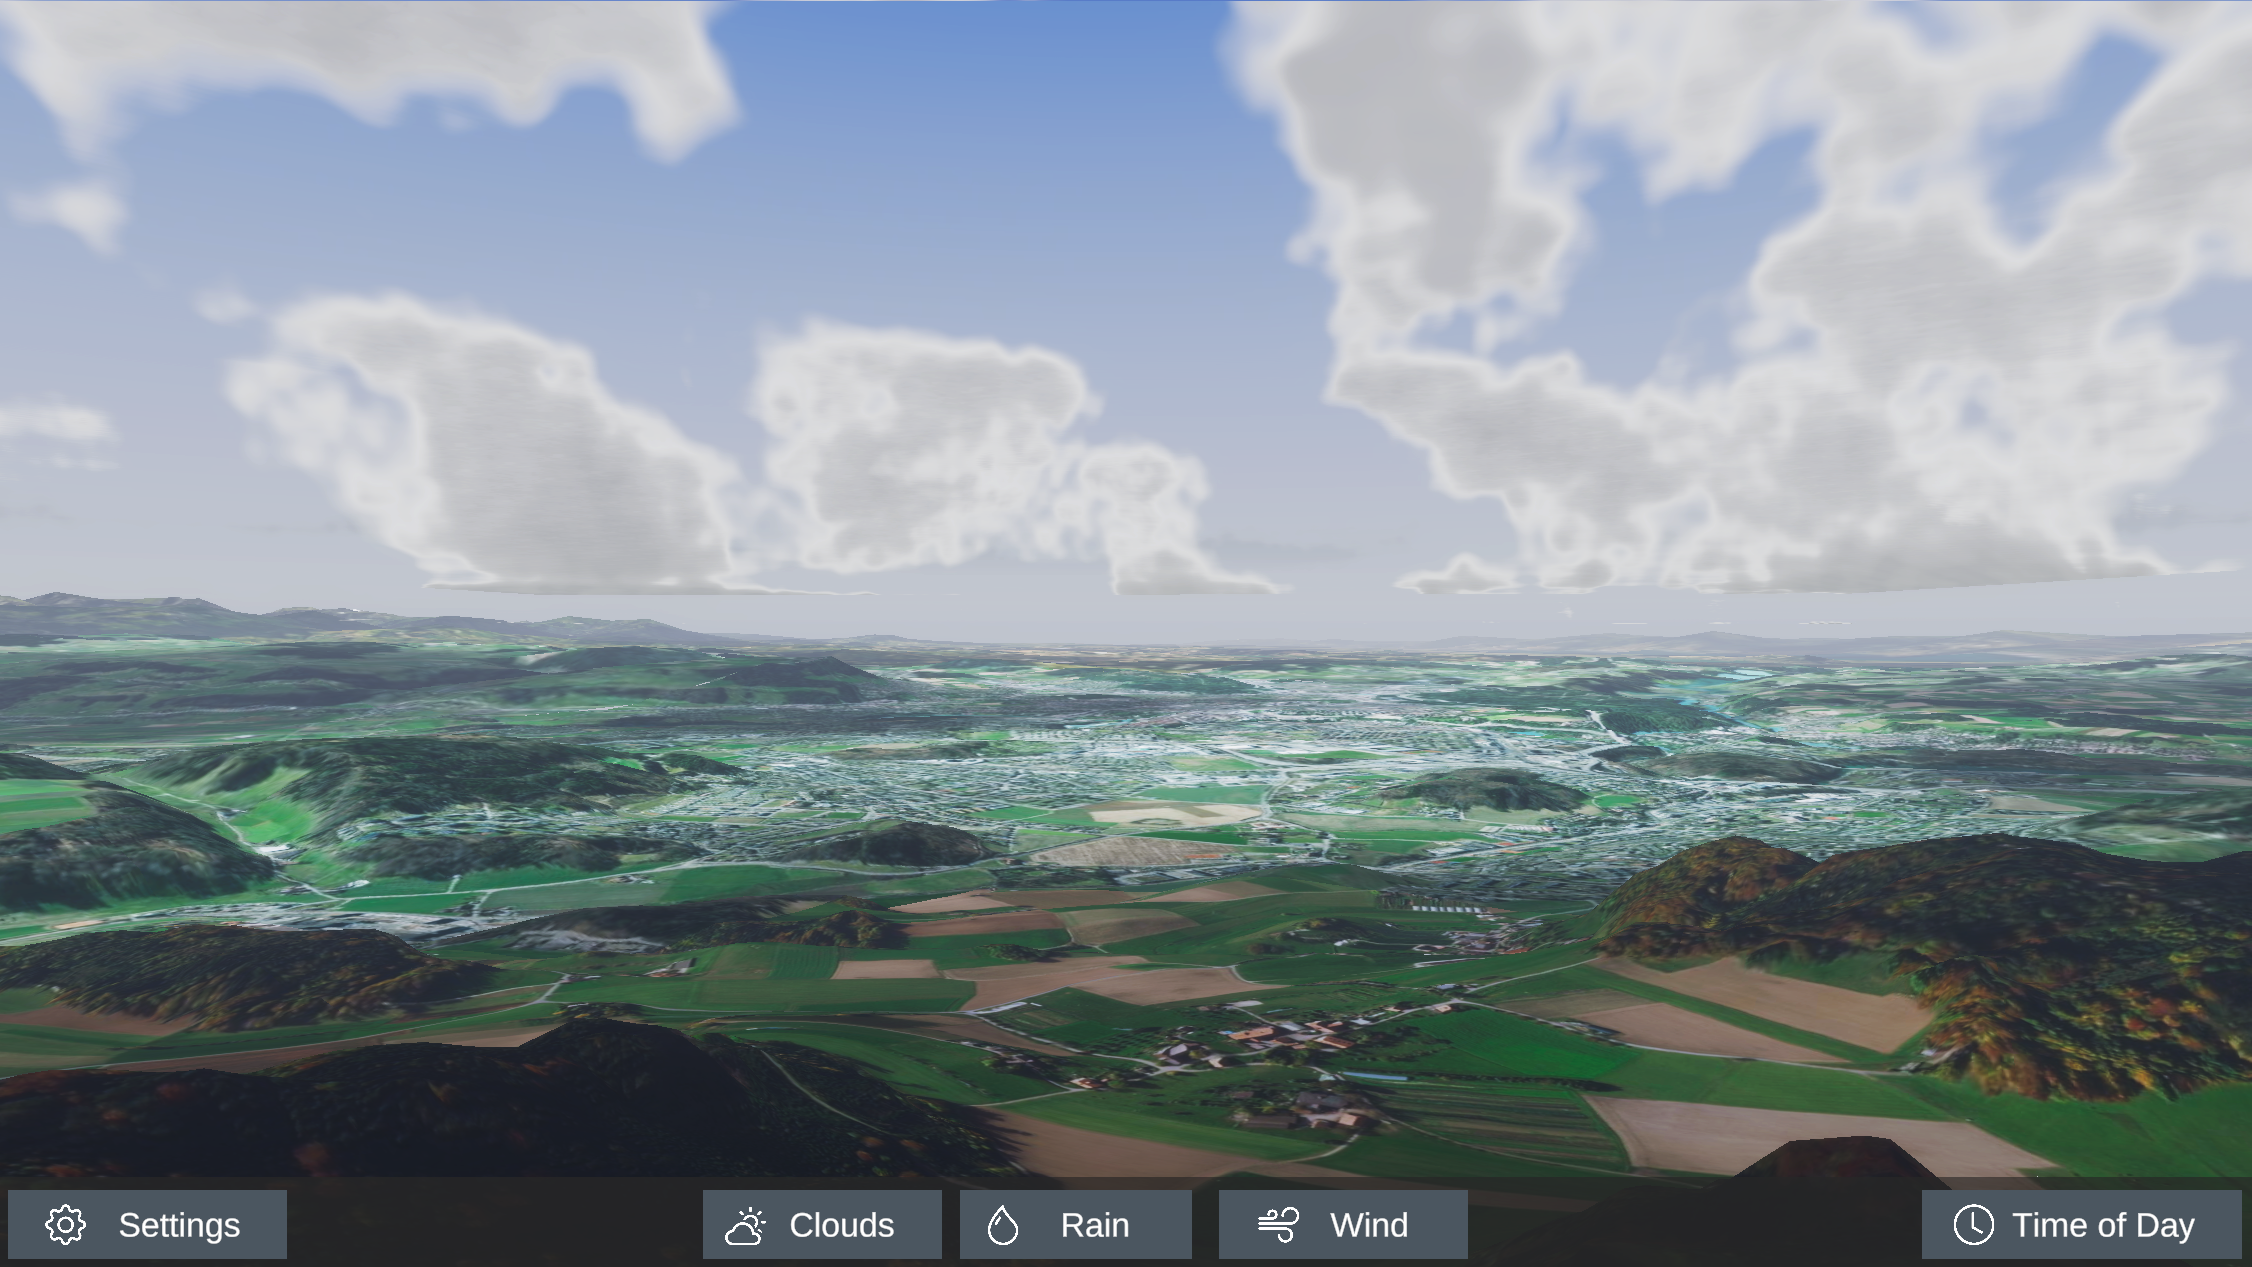
\includegraphics[width=\linewidth]{results/wheel2.png}
            \captionof{figure}{Final render output of weather rendering system.}
            \label{img:msfs:2}
        \end{minipage}
\end{figure}

\noindent
The comparison shows that the colors of the environment is just as important as the realism of the clouds.
For example, the vibrant colors towards the horizon in \autoref{img:msfs:1} give the scene a much more natural appearance.

\subsection{Conclusion}
The rendered results bring out the most of the capabilities of the weather rendering system and show many diverse scenarios.
Especially so when rendering the weather during a sunrise or sunset. The sun light strongly emphasizes the volumetric properties of the clouds.
\emptyline
As \sectionref{section:eval:measurability} already states, there is no practical method of measuring the realism of the weather rendering system.
Hence, for this project, the only suitable method to assess the realism of a rendered image, that still conforms to the scope of the project, is comparing the \gls{inengine} render side-by-side with the \emph{Roundshot} image.